\appendix
\chapter{Anhang}
Appendix
\section{Graph-Datenbanken - Grundlegende technologische Aspekte}
\section{Graph-Datenbanken und -Frameworks - Ausgewählte Systeme}
\begin{figure}[H]

    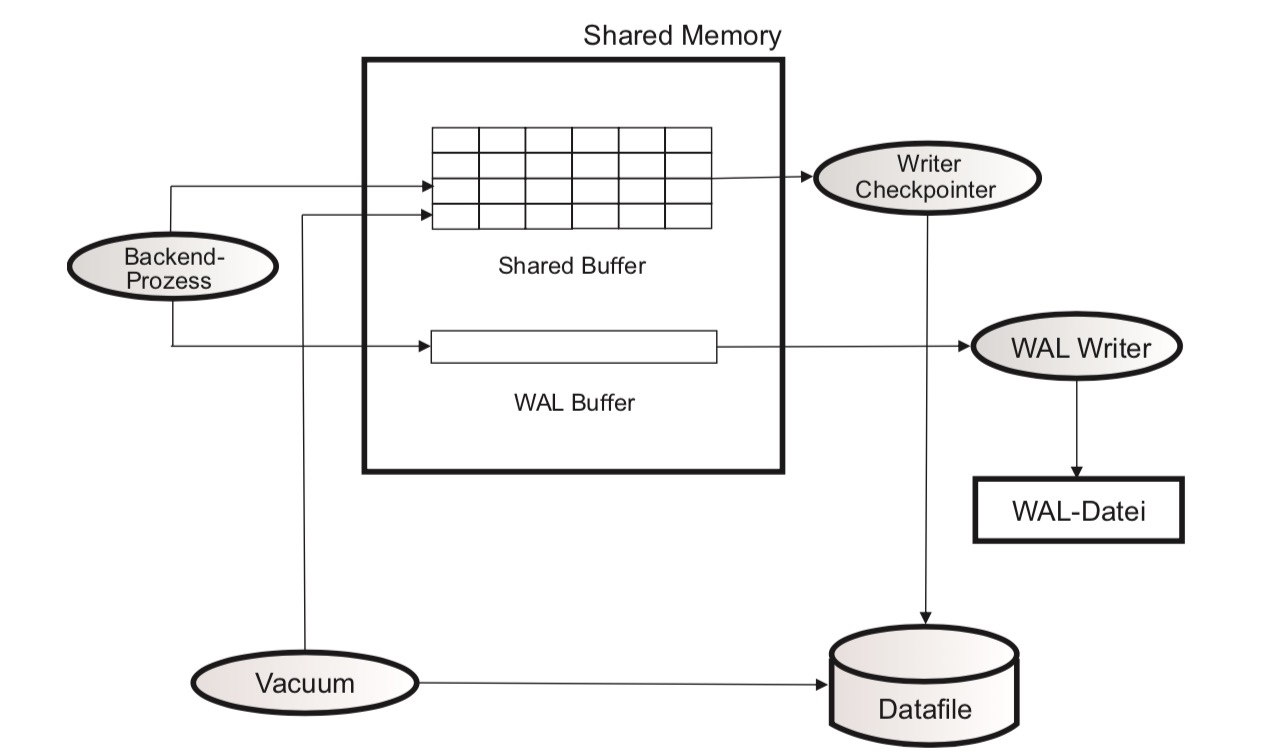
\includegraphics[width = \linewidth]{images/postgresArchitektur.jpg}
    \caption{Postgres Architektur}
    \label{Postgres Architektur}

\end{figure}
\section{Graph-Datenbanken im praktischen Einsatz: OLTP}
\lstsetsql
\begin{lstlisting}[language=SQL,caption=CSV Input,frame=single, label={copy}]
    \copy Beitraege
    FROM './data/Beitraege.csv' DELIMITER ',' CSV HEADER;
\end{lstlisting}

\begin{lstlisting}[language=SQL,caption=Anlegen der Tabelle facebook-profiles,frame=single]
    CREATE TABLE public."facebook-profiles"
    (
        id serial PRIMARY KEY,
        first TEXT,
        last TEXT,
        gender TEXT,
        country TEXT,
        birth TEXT
    );
\end{lstlisting}

\begin{lstlisting}[language=SQL,caption=Anlegen der Tabelle facebook,frame=single]
    CREATE TABLE public.facebook
    (
        src INT,
        dst INT,
        type TEXT,
        date TEXT
    );
\end{lstlisting}

\begin{lstlisting}[language=SQL,caption=Hinzufügen von Fremdschlüsseln,frame=single, label={foreignKey}]
    \copy profiles_facebook_tmp(first,last,gender,birth,country) FROM '/data/WS2018/facebook-profiles' DELIMITER ',' CSV HEADER;
    INSERT INTO profiles_facebook (ID, first, last, gender, birth, country)
    SELECT ID-1, first, last, gender, birth, country from profiles_facebook_tmp;
\end{lstlisting}

\begin{lstlisting}[language=SQL,caption = Verschachteltes SELECT Statement,frame=single,label={SELECT} ]
    SELECT DISTINCT(dst) FROM team22.relation_facebook WHERE src IN(
        SELECT DISTINCT(dst) FROM team22.relation_facebook WHERE src IN(
            SELECT DISTINCT(dst)FROM team22.relation_facebook WHERE src IN(1)
        )
    )
\end{lstlisting}

\begin{lstlisting}[language=SQL,caption = Rekursiver JOIN,frame=single, label={JOIN} ]
    SELECT DISTINCT(rf3.dst)
    FROM public.relation_facebook rf1,
    public.relation_facebook rf2,
    public.relation_facebook rf3
    WHERE rf2.src = rf1.dst
    AND rf3.src = rf2.dst
    AND rf1.src = 765;
\end{lstlisting}
\newpage
\begin{lstlisting}[language=SQL,caption = Selbstgeschriebenes Stored Procedure,frame=single, label={recursiveFunction} ]
    CREATE OR REPLACE FUNCTION recursivesearch(tInput integer[], iRecursionDepth integer, sTable text) RETURNS SETOF integer AS $$
    Declare
    intermDst_ integer[];
    iCount integer;
    BEGIN
    --iRecursionDepth = iRecursionDepth + 1;
    CREATE TEMPORARY TABLE intermDst AS SELECT * FROM unnest(tInput);
    EXECUTE 'CREATE TEMPORARY TABLE intermDst1 AS SELECT DISTINCT(dst) FROM ' || sTable || ' WHERE src IN (SELECT * FROM intermDst)';
    -- Does not return from function!
    return query SELECT * FROM intermDst1;
    -- Does not return from function!
    intermDst_ := ARRAY(SELECT * FROM intermDst1);
    raise notice 'timestamp: %', clock_timestamp();
    SELECT count(*) INTO iCount FROM intermDst;
    raise notice 'Count Table: %', iCount;
    DROP TABLE intermDst;
    DROP TABLE intermDst1;
    -- As recursion depth is 5
    if iRecursionDepth > 1 THEN
    return query SELECT * FROM recursivesearch(intermDst_, iRecursionDepth - 1, sTable);
    ELSE
    RETURN;
    END IF;
    END;
    $$ LANGUAGE plpgsql;
\end{lstlisting}

\begin{lstlisting}[language=SQL,caption = SQL Standard SQL Mittel,frame=single, label={StandardSQL} ]
    CREATE OR REPLACE FUNCTION selectWithUnionSourceCodeGenerator_withStartingNode(sTable text, startingNode integer ) RETURNS SETOF integer AS $$
    Declare
    intermDst_ integer[];
    tStatement text;
    tSelectStatement text;
    tWithStatement text;
    tUnionStatement text;
    tWithStatementClose text;
    BEGIN
    tWithStatement := 'WITH RECURSIVE graphtraverse AS(';
    tSelectStatement := 'SELECT DISTINCT(dst) FROM ' || sTable || ' WHERE src ='||startingNode;
    tUnionStatement := ' UNION SELECT DISTINCT(p.dst) FROM ' || sTable || ' p WHERE src IN (p.src)';
    tWithStatementClose := ') SELECT * FROM graphtraverse';
    tStatement := tWithStatement || tSelectStatement || tUnionStatement || tWithStatementClose;
    raise notice 'Execute String %', tStatement;
    return query EXECUTE tStatement;
    END;
    $$ LANGUAGE plpgsql;
\end{lstlisting}

\section{Graph-Datenbanken im praktischen Einsatz: OLAP}
%\chapter{Anhang}
%Appendix